\documentclass{article}
\usepackage[utf8]{inputenc}
\usepackage{amsmath, esint}
\usepackage{wasysym}
\usepackage{qrcode}
\usepackage[colorlinks]{hyperref}
\usepackage{lmodern}
\usepackage{graphicx}
\usepackage{xcolor}
\usepackage[left=2cm, top=3cm, right=2cm]{geometry}
\usepackage{minted}
\usepackage{booktabs}
\usepackage{svg}
\usepackage{xcolor}
\definecolor{LightGray}{gray}{0.975}

%setup new colors
\hypersetup{
%linkcolor=blue
%,citecolor=
%,filecolor=
urlcolor=blue
%,menucolor=
%,runcolor=
%,linkbordercolor=
%,citebordercolor=
%,filebordercolor=
%,urlbordercolor=
%,menubordercolor=
%,runbordercolor=
}

\title{Databases \\ Lab 02: A `gentle' Introduction to Basic SQL.}
\author{Andrés Oswaldo Calderón Romero, Ph.D.}
\date{\today}

\begin{document}

\maketitle

\section{Introduction}
In this lab, you will strengthen your understanding of basic SQL through a combination of guided resources and hands-on practice. We will begin by revisiting the core concepts discussed in class using short video tutorials and interactive exercises from W3Schools. These activities will provide a structured review of SQL syntax, selection, filtering, aggregation, and other foundational operations, ensuring you are comfortable with the essential commands before moving on to more complex tasks.

Once familiar with the basics, you will apply your skills using the \texttt{university} database from the Database System Concepts book. You will load a smaller version of this database into PostgreSQL and run a series of queries that combine SQL coding, relational algebra expressions, and output verification. This practical component will help you bridge the gap between theoretical knowledge and actual database manipulation, preparing you for more advanced SQL topics in future labs.

Let's go!

\section{W3Schools SQL YouTube Videos}
We will watch a YouTube playlist from the \href{https://www.youtube.com/@w3schools}{W3Schools.com} channel covering introductory SQL. You can access the playlist \href{https://youtube.com/playlist?list=PLP9IO4UYNF0UQkBXlTMSw0CYsxv-GDkkI&si=qel9VClPHmerhGlz}{here}. If you prefer, you can enable Spanish subtitles via the Settings button. The playlist consists of 11 short videos. Simply watch them—there is no specific assignment or submission required for now.

\section{W3Schools Interactive SQL Tutorial}
Now, you will go through the interactive SQL tutorial on the W3Schools website. First, create a free account. The tutorial begins \href{https://www.w3schools.com/sql/}{here}. You will find several lessons listed in the left panel. You only need to complete the following:

\begin{itemize}
  \item Intro
  \item Syntax
  \item Select
  \item Select Distinct
  \item Where
  \item Order By
  \item And
  \item Or
  \item Not
  \item Null Values
  \item Aggregate Functions
  \item Min and Max
  \item Count
  \item Sum
  \item Avg
  \item Like
  \item Wildcards
  \item In
  \item Between
  \item Aliases
\end{itemize}

Once you have completed all the lessons, take a screenshot similar to Figure~\ref{fig:panel}. Make sure your profile picture and your progress (green line in the left panel) are clearly visible. Each team member must provide their own screenshot.

\begin{figure}[t]
 \centering
 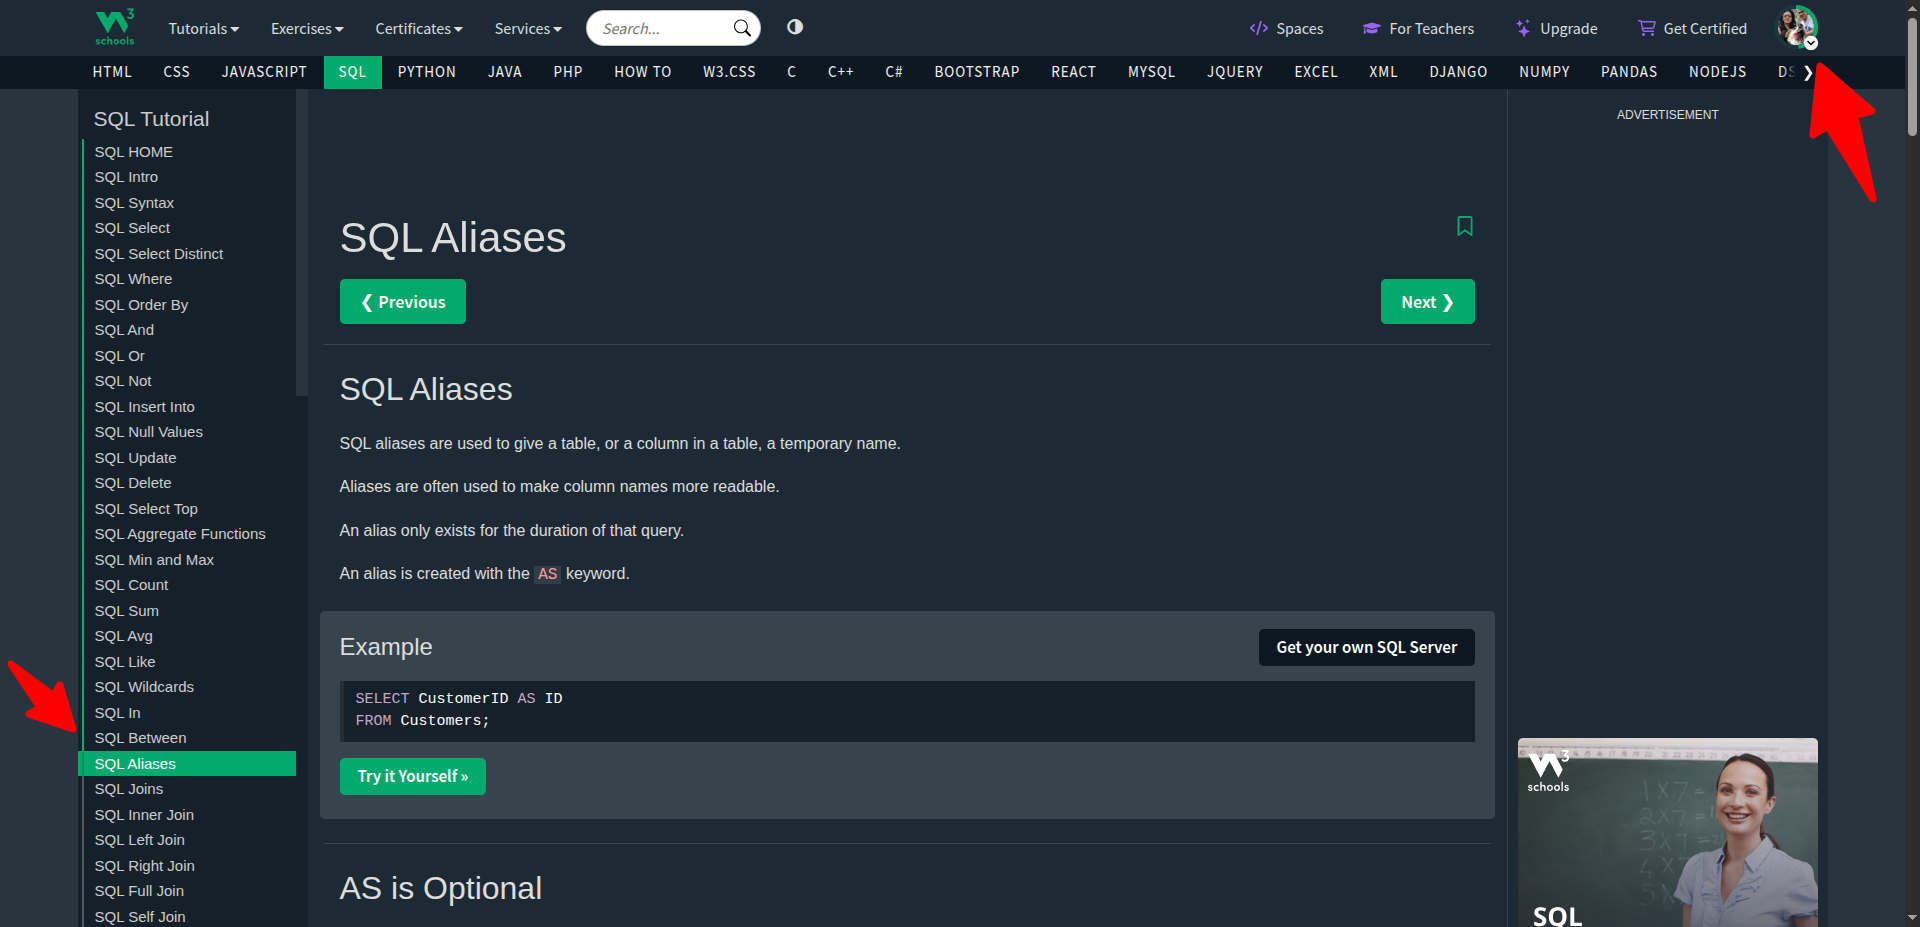
\includegraphics[width=\textwidth]{figures/w3sql}
 \caption{Lessons panel displayed in the W3Schools SQL Tutorial, showing progress tracking in the left sidebar.}
 \label{fig:panel}
\end{figure}

\section{The \texttt{university} Database}
The website for the book \textit{Database System Concepts} provides backups of the \texttt{university} database we have been using in class. We will load a smaller version into PostgreSQL so we can practice the SQL statements we have already learned. You will need to download the following two files:

\begin{enumerate}
  \item The \href{https://db-book.com/university-lab-dir/sample_tables-dir/DDL.sql}{\texttt{DDL.sql}} file, which contains the code to create the database structure.
  \item The \href{https://db-book.com/university-lab-dir/sample_tables-dir/smallRelations/smallRelationsInsertFile.sql}{\texttt{smallRelationsInsertFile.sql}} file, which contains the code to populate the database with the same records used in the examples from the book.
\end{enumerate}

Download both files and place them in the same folder. We will assume that you already have a functional PostgreSQL instance running on your machine. You should be able to access a PostgreSQL console similar to Figure~\ref{fig:psql}.

\begin{figure}
 \centering
 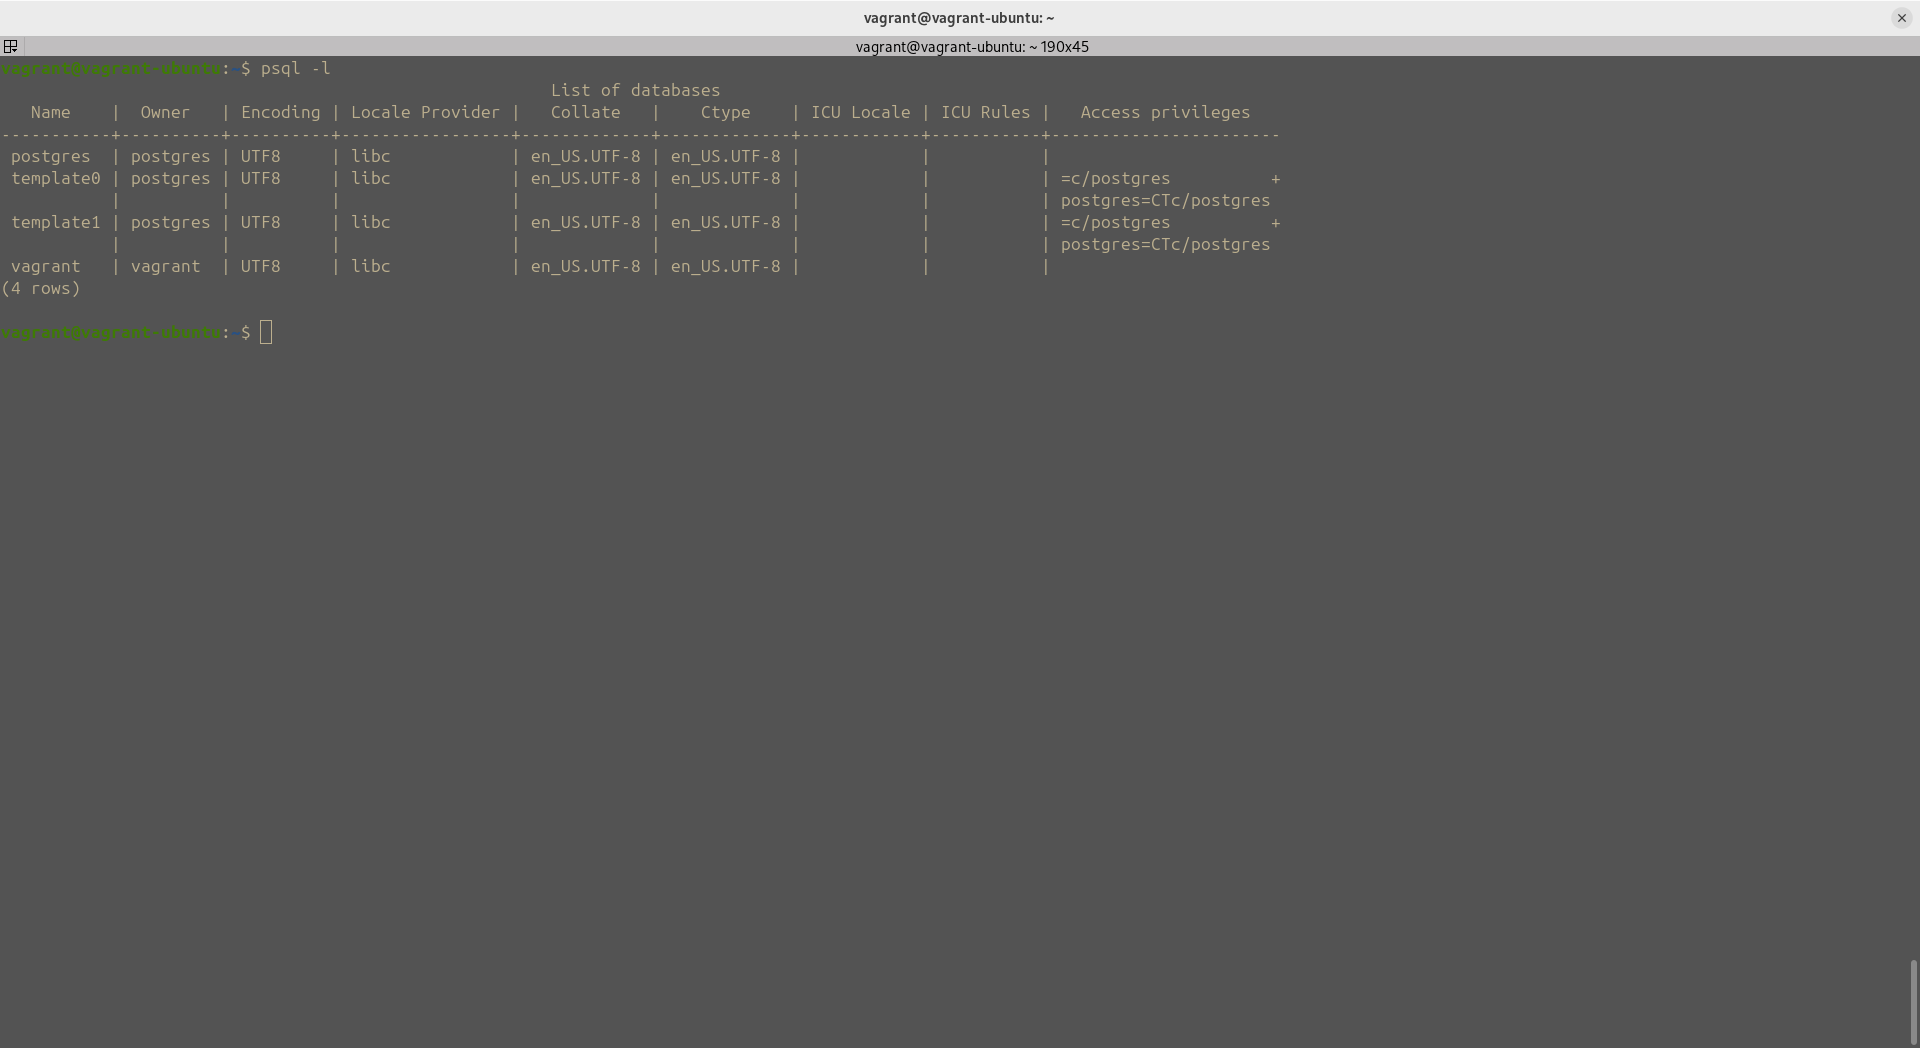
\includegraphics[width=\textwidth]{figures/psql}
 \caption{Ensure that PostgreSQL is installed on your system.}
 \label{fig:psql}
\end{figure}

First, create a database named \texttt{university}:

\begin{minted}
[tabsize=4, obeytabs, frame=lines, framesep=2mm, baselinestretch=1.2, bgcolor=LightGray, fontsize=\footnotesize]{bash}
createdb university
\end{minted}

Next, connect to the newly created database:

\begin{minted}
[tabsize=4, obeytabs, frame=lines, framesep=2mm, baselinestretch=1.2, bgcolor=LightGray, fontsize=\footnotesize]{bash}
psql university
\end{minted}

You are now in the PostgreSQL prompt. From here, use the \texttt{\textbackslash i} command to load the schema and data for the database. Remember to update the file paths to match the location where you saved the downloaded files.

First, load the \texttt{DDL.sql} file:

\begin{minted}
[tabsize=4, obeytabs, frame=lines, framesep=2mm, baselinestretch=1.2, bgcolor=LightGray, fontsize=\footnotesize]{bash}
\i /path_to_files/DDL.sql
\end{minted}

Then, load the \texttt{smallRelationsInsertFile.sql} file:

\begin{minted}
[tabsize=4, obeytabs, frame=lines, framesep=2mm, baselinestretch=1.2, bgcolor=LightGray, fontsize=\footnotesize]{bash}
\i /path_to_files/smallRelationsInsertFile.sql
\end{minted}

And that’s it! You’re all set. Let’s run a quick SQL query to test:

\begin{minted}
[tabsize=4, obeytabs, frame=lines, framesep=2mm, baselinestretch=1.2, bgcolor=LightGray, fontsize=\footnotesize]{sql}
SELECT * FROM instructor;
\end{minted}

You are now ready to explore the SQL queries we have already covered in class. If you encounter any issues, watch this \href{https://youtu.be/2hco9E1R6K8}{video}, which provides a detailed walkthrough of how to load the schema and data for the \texttt{university} database.

\section{Independent Work} \label{sec:work}
With the \texttt{university} database prepared, proceed to execute and answer the following queries:

\begin{enumerate}
  \item Retrieve the names of all instructors, along with their department names and the corresponding department building names.
  \item For all instructors in the university who have taught at least one course, find their names and the course IDs of all courses they taught.
  \item Find the names of all departments whose building name contains the substring \texttt{Watson}.
  \item Find the set of all courses taught in both the Spring 2018 semester and the Fall 2017 semester.
  \item Find all instructors who appear in the \texttt{instructor} relation with a \texttt{NULL} value for salary.
  \item Find the average salary in each department.
  \item Show the departments where the average salary of instructors is greater than \$42{,}000.
  \item Find the titles of courses in the \texttt{Comp. Sci.} department that have 3 credits.
  \item Find the enrollment of each section that was offered in Fall 2017.
  \item Find the names of all instructors whose salary is greater than that of every instructor in the Biology department.
  \item Propose your own query and solve it using SQL.
\end{enumerate}

For each query, you must provide its corresponding \textit{relational algebra} expression, the \texttt{SQL} code, and the query result (either a copy–paste of the output or a screenshot).

We expect a well-structured report in \textbf{PDF} format containing the requested information from the previous sections. Additionally, include a plain-text file with extension \texttt{.sql} that contains all the statements from Section~\ref{sec:work}. Package both files (\texttt{.pdf} and \texttt{.sql}) into a single \textbf{ZIP} file and submit it via Brightspace. The submission deadline is \textbf{August 27, 2025}.


\vspace{5mm}
Happy Hacking! \includesvg[width=4mm]{figures/sunglasses}

\end{document}
